

En clase se describió el Lema de Ito para determinar el precio futuro de los activos con riesgo. El modelo resultante fue el siguiente:
\[
S_T = S_0 e^{\left(\mu - \frac{\sigma^2}{2}\right)(T-t) + \sigma\sqrt{T-t}\varepsilon_t}
\]

\vspace{0.5cm}

% Subsección A
\subsubsection*{{a. Componentes de la ecuación}}
Explique con palabras \textbf{\textit{no técnicas}} cada uno de los componentes de esta ecuación.
    
\vspace{0.3cm}
\begin{itemize}[label={$\circ$}, itemsep=0.3cm, leftmargin=1cm]
    \item $S_T$: \textbf{El precio futuro del activo.} Es el destino al que queremos llegar, es decir, el valor final que tendrá la acción en la fecha futura.
    \item $\left(\mu - \frac{\sigma^2}{2}\right)(T-t)$: \textbf{El crecimiento seguro.} Lo que esperamos ganar por el simple paso del tiempo, descontando el desgaste que causa la volatilidad.
    \item $\sigma\sqrt{T-t}\varepsilon_t$: \textbf{El factor suerte.} Representa el impacto total de las noticias imprevistas y los eventos aleatorios. Es la parte impredecible que sube o baja el precio.
    \item $e^{\left(\mu - \frac{\sigma^2}{2}\right)(T-t) + \sigma\sqrt{T-t}\varepsilon_t}$: \textbf{El multiplicador de crecimiento total.} Junta la tendencia segura y el factor suerte para darnos el número final por el que multiplicamos nuestro precio inicial ($S_0$).
\end{itemize}

\vspace{0.5cm}

% Subsección B
\subsubsection*{{b. Diagrama de flujo}}
Estando en febrero de 2026, realice un \textbf{diagrama de flujo} que describa el proceso para estimar el precio de un activo al cierre del año 2026.
    
\vspace{0.2cm}
\begin{figure}[h]
\centering
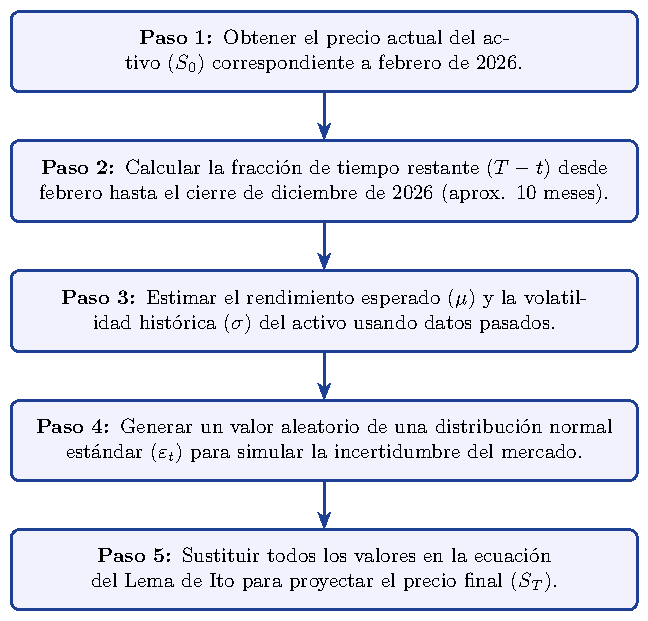
\includegraphics[width=0.5\textwidth]{Diagrama.pdf}
\caption{Flujo del modelo}
\end{figure}
\vspace{0.5cm}

% Subsección C
\subsubsection*{{c. Estimación del valor del portafolio}}
Estando en febrero de 2026, estime para el cierre del año 2026 el \textbf{valor del portafolio} elegido en la pregunta IV.
    
\vspace{0.2cm}
\noindent \textcolor{gray}{\textit{* La estimación y el desarrollo de este punto se encuentran detallados en la presentación \textbf{portafolio 1}.}}

\vspace{0.5cm}

% Subsección D
\subsubsection*{{d. VaR y CVaR del portafolio}}
Estando en febrero de 2026, obtenga el VaR y el CVaR al 97.5\% de confianza de este portafolio al cierre de diciembre de 2026. Explique ampliamente.
    
\vspace{0.2cm}
\noindent \textcolor{gray}{\textit{* El cálculo y la explicación amplia del VaR y CVaR se encuentran en la presentación \textbf{portafolio 1}.}}
